\documentclass[11pt,oneside,letterpaper]{article}

% graphicx package, useful for including eps and pdf graphics
\usepackage{graphicx}
\DeclareGraphicsExtensions{.pdf,.png,.jpg}

% basic packages
\usepackage{color} 
\usepackage{parskip}
\usepackage{float}

% text layout
\usepackage{geometry}
\geometry{textwidth=15cm} % 15.25cm for single-space, 16.25cm for double-space
\geometry{textheight=22cm} % 22cm for single-space, 22.5cm for double-space

% helps to keep figures from being orphaned on a page by themselves
\renewcommand{\topfraction}{0.85}
\renewcommand{\textfraction}{0.1}

% bold the 'Figure #' in the caption and separate it with a period
% Captions will be left justified
\usepackage[labelfont=bf,labelsep=period,font=small]{caption}

% review layout with double-spacing
%\usepackage{setspace} 
%\doublespacing
%\captionsetup{labelfont=bf,labelsep=period,font=doublespacing}

% cite package, to clean up citations in the main text. Do not remove.
\usepackage{cite}
%\renewcommand\citeleft{(}
%\renewcommand\citeright{)}
%\renewcommand\citeform[1]{\textsl{#1}}

% Remove brackets from numbering in list of References
\renewcommand\refname{\large References}
\makeatletter
\renewcommand{\@biblabel}[1]{\quad#1.}
\makeatother

\usepackage{authblk}
\renewcommand\Authands{ \& }
\renewcommand\Authfont{\normalsize \bf}
\renewcommand\Affilfont{\small \normalfont}

% comments
\usepackage{ulem}
\definecolor{blue}{rgb}{0.324,0.609,0.708}
\definecolor{purple}{rgb}{0.459,0.109,0.538}
\def\tb#1#2{\sout{#1} \textcolor{purple}{#2}} 
\def\tbc#1{\textcolor{purple}{[#1]}}
\def\ms#1#2{\sout{#1} \textcolor{blue}{#2}} 
\def\msc#1{\textcolor{blue}{[#1]}}

% notation
\usepackage{amsmath}
\usepackage{amssymb}
\newcommand{\virus}{\mathbf{x}}						% virus coordinate
\newcommand{\serum}{\mathbf{y}}						% serum coordinate
\newcommand{\viruses}{\mathbf{X}}					% set of virus coordinates
\newcommand{\sera}{\mathbf{Y}}						% set of serum coordinates
\newcommand{\ve}{v}									% virus effect
\newcommand{\se}{s}									% serum effect
\newcommand{\ves}{\mathbf{v}}						% set of virus effects
\newcommand{\ses}{\mathbf{s}}						% set of serum effects
\newcommand{\point}{f_{\scriptscriptstyle \vert}}	% point likelihood
\newcommand{\threshold}{f_{\textstyle \lrcorner}}	% threshold likelihood
\newcommand{\interval}{f_{\sqcup}}					% interval likelihood
\newcommand{\mdssd}{\varphi}						% MDS standard deviation
\newcommand{\virussd}{\sigma_x}						% virus / diffusion standard deviation
\newcommand{\serumsd}{\sigma_y}						% serum standard deviation
\newcommand{\tree}{\tau}							% phylogeny
\newcommand{\vn}{n}									% number of viruses
\newcommand{\sn}{k}									% number of sera
\newcommand{\normal}{\mathcal{N}}					% normal distribution
\newcommand{\bwithin}{\beta_c}						% within clade drift coefficient
\newcommand{\bsister}{\beta_s}						% sister clade drift coefficient
\newcommand{\bother}{\beta_t}						% across clade drift coefficient
\newcommand{\driftclade}[1]{x_\mathrm{#1}}
\setlength{\arraycolsep}{2pt}
\newcommand{\smalltwomatrix}[2]{\scriptsize \Big( \begin{matrix} #1 \\ #2 \end{matrix} \Big)}				% pretty inline matrix 
\newcommand{\smallfourmatrix}[4]{\scriptsize \Big( \begin{matrix} #1 & #2 \\ #3 & #4 \end{matrix} \Big)}	% pretty inline matrix 
\newcommand{\twomatrix}[2]{\left( \begin{matrix} #1 \\ #2 \end{matrix} \right)}								% pretty inline matrix 
\newcommand{\fourmatrix}[4]{\left( \begin{matrix} #1 & #2 \\ #3 & #4 \end{matrix} \right)}					% pretty inline matrix 

%%% TITLE %%%
\title{\vspace{1.0cm} \LARGE \bf 
Supporting Text: \\
Integrating influenza antigenic dynamics with molecular evolution
}

\author[1]{Trevor Bedford}
\author[2,3,4]{Marc A. Suchard}
\author[5]{Philippe Lemey}
\author[1]{Gytis Dudas}
\author[6]{Victoria Gregory}
\author[6]{Alan J. Hay}
\author[6]{John W. McCauley}
\author[7]{Colin A. Russell}
\author[7,8]{Derek J. Smith}
\author[1,9]{Andrew Rambaut}

\affil[1]{Institute of Evolutionary Biology, University of Edinburgh, Edinburgh, UK}
\affil[2]{Department of Biomathematics, David Geffen School of Medicine at UCLA, University of California, Los Angeles CA, USA}
\affil[3]{Department of Human Genetics, David Geffen School of Medicine at UCLA, University of California, Los Angeles CA, USA}
\affil[4]{Department of Biostatistics, UCLA Fielding School of Public Health, University of California, Los Angeles CA, USA}
\affil[5]{Department of Microbiology and Immunology, Katholieke Universiteit Leuven, Leuven, Belgium}
\affil[6]{Division of Virology, MRC National Institute for Medical Research, Mill Hill, London, UK}
\affil[7]{Department of Zoology, University of Cambridge, Cambridge, UK.}
\affil[8]{Department of Virology, Erasmus Medical Centre, Rotterdam, Netherlands.}
\affil[9]{Fogarty International Center, National Institutes of Health, Bethesda, MD, USA.}

\date{}

\begin{document}

\maketitle

%%% SUPPORTING METHODS %%%
\section*{Supporting Methods}

\subsection*{Antigenic cartography}

Antigenic characteristics of viral strains are often assessed through immunological assays such as the hemagglutination inhibition (HI) assay \cite{Hirst43}.  
At heart, these assays compare the reactivity of one virus strain to antibodies raised against another virus strain via challenge or vaccination.  
In the case of HI, the measurement of cross-reactivity takes the form of a titer representing the dilution factor at which serum raised against a particular virus ceases to be effective at inhibiting the binding of another virus to red blood cells.  
These factors are commonly assessed by serial dilution, so that HI titers will form a log series, 40, 80, 160, etc \dots.
Because experimental HI titers typically differ by factors of two, we find it convenient to work in log$_2$ space and represent the titer of virus $i$ against serum $j$ as $H_{ij} = \mathrm{log}_2 \mbox{(HI titer)}$, i.e.\ a titer of 160 has $H_{ij} = 7.32$.
Due to experimental constraints, most comparisons cannot be made, leading to a sparse observation matrix $\mathbf{H} = \{H_{ij}\}$.  
Further, measurements are usually interval and truncated, e.g.\ inhibition may cease somewhere between the serial titers of 160 and 320, or inhibition may be absent at all titers assayed, suggesting a threshold somewhere between 0 and 40.  

Previous work \cite{Smith04, Cai10} has used multidimensional scaling to place viruses and sera on an `antigenic map'.  
These methods heuristically optimize locations of viruses and sera by seeking to minimize the sum of squared errors between titers predicted by map locations and observed titers.  
Antigenic maps produced by these methods have proved useful in categorizing virus phenotypes \cite{Smith04}, but the extension of these methods to integrate genetic data remains notably lacking.

Here, we follow previous models in representing antigenic locations as points in a low $P$-dimensional antigenic map. 
One of our initial goals is to find an optimal projection of the high-dimensional distance matrix $\mathbf{H}$ into this lower dimensional space. 
We conduct this projection using Bayesian multidimensional scaling (BMDS) \cite{Oh01} in which we construct a probabilistic model to quantify the fit of a particular configuration of cartographic locations to the observed matrix of serological measurements.
Typically, $P = 2$, but higher or lower dimensions may better reflect the data. 

Let $\virus_i \in \mathbb{R}^{P}$ represent the cartographic location of virus $i$ for $i = 1,\ldots,\vn$, so that $\virus_i = (x_{i1}, x_{i2})^{\prime}$ for $P=2$. 
Similarly, let $\serum_j$ represent the cartographic location of serum $j$ for $j = 1,\ldots,\sn$, so that $\serum_j = (y_{j1},y_{j2})^{\prime}$ for $P=2$.
For notational compactness, we collect together all virus coordinates into an $\vn \times P$ matrix  $\viruses = (\virus_1, \ldots, \virus_{\vn})^{\prime}$ and all serum coordinates into an $\sn \times P$ matrix $\sera = (\serum_{1},\ldots,\serum_{\sn})^{\prime}$.
Virus and serum may be isolated from / raised against the same strain and have different cartographic locations, and separate serum isolates raised against the same strain may also have different cartographic locations. 
This gives a set of distances between virus and serum cartographic locations 
\begin{equation}
	\delta_{ij} =  || \virus_i - \serum_j ||_2,
\end{equation}
where $|| \cdot ||_2$ is an $L_2$ norm.

Traditional approaches to antigenic cartography \cite{Smith04} begin by defining immunological distance as
\begin{equation}
	d_{ij} =  \se_j - H_{ij},
\end{equation}
where $H_{ij}$ is the log$_2$ titer of virus $i$ against serum $j$ and serum effect $\se_j = \max ( H_{1j},\ldots,H_{\vn j} )$ is fixed.
In following multidimensional scaling (MDS), these approaches attempt to optimize over unknown $\viruses$ and $\sera$ such that
\begin{equation}
	\sum_{(i,j) \in \cal I} 
	\left(
		\delta_{ij} - d_{ij}
	\right)^2
\end{equation}
is minimized, where $\mathcal{I} = \{ (i,j) : H_{ij} \mbox{ is measured} \}$.

Here, we instead assume a probabilistic interpretation in which an observed titer is normally distributed around its cartographic expectation with variance $\mdssd^2$,
\begin{equation} \label{hij}
	H_{ij} \sim \normal( \se_j - \delta_{ij}, \, \mdssd^2 ).
\end{equation}
Consequently, the likelihood of observing an exact titer given the placement of antigenic locations is 
\begin{equation} 
	\point(H_{ij}) = \phi \left( \frac{ H_{ij} + \delta_{ij} - \se_j }{ \mdssd } \right),
\end{equation}
where $\phi(\cdot)$ represents the standard normal probability density function (PDF).
Previous BMDS has employed a sampling density truncated to strictly positive quantities since $d_{ij}$ are directly observed, non-negative quantities.  
In the antigenic setting, these remain random and can be negative since neither $\se_j$ is known nor is $H_{ij}$ observed with much precision. 

HI assays sometimes show no inhibition at all measured titrations, e.g.\ a measurement can be reported as `$<$40'.
In this case, the likelihood of observing the threshold measurement follows the cumulative density of the lower tail of the normal distribution
\begin{equation} 
	\threshold(H_{ij}) = \Phi \left( \frac{ H_{ij} + \delta_{ij} - \se_j }{ \mdssd } \right),
\end{equation}
where $\Phi(\cdot)$ represents the standard normal cumulative distribution function (CDF).
Although it is simplest to assume that immunological measurements represent point estimates, it seems more natural to assume that the threshold for inhibition occurs between two titers, e.g.\ we observe inhibition at 1:160 dilution and no inhibition at 1:320 dilution.
Rather than taking the HI titer as 160, we can instead treat this as an interval measurement, assuming that the exact titer for inhibition would occur somewhere between 160 and 320.
HI titers are usually reported as the highest titer that successfully inhibits virus binding, so that in this case, we calculate the likelihood of an interval measurement as
\begin{equation} 
	\interval(H_{ij}) = \Phi \left( \frac{ H_{ij} + \delta_{ij} - \se_j + 1 }{ \mdssd } \right) - \Phi \left( \frac{ H_{ij} + \delta_{ij} - \se_j }{\mdssd} \right).
\end{equation}
These likelihoods are illustrated in Figure~\ref{hij_likelihood}.
Throughout our analyses, we use interval likelihoods $\interval$ rather than point likelihoods $\point$ unless otherwise noted.

%%% hij_likelihood %%%
\begin{figure}[tb]
	\centering		
	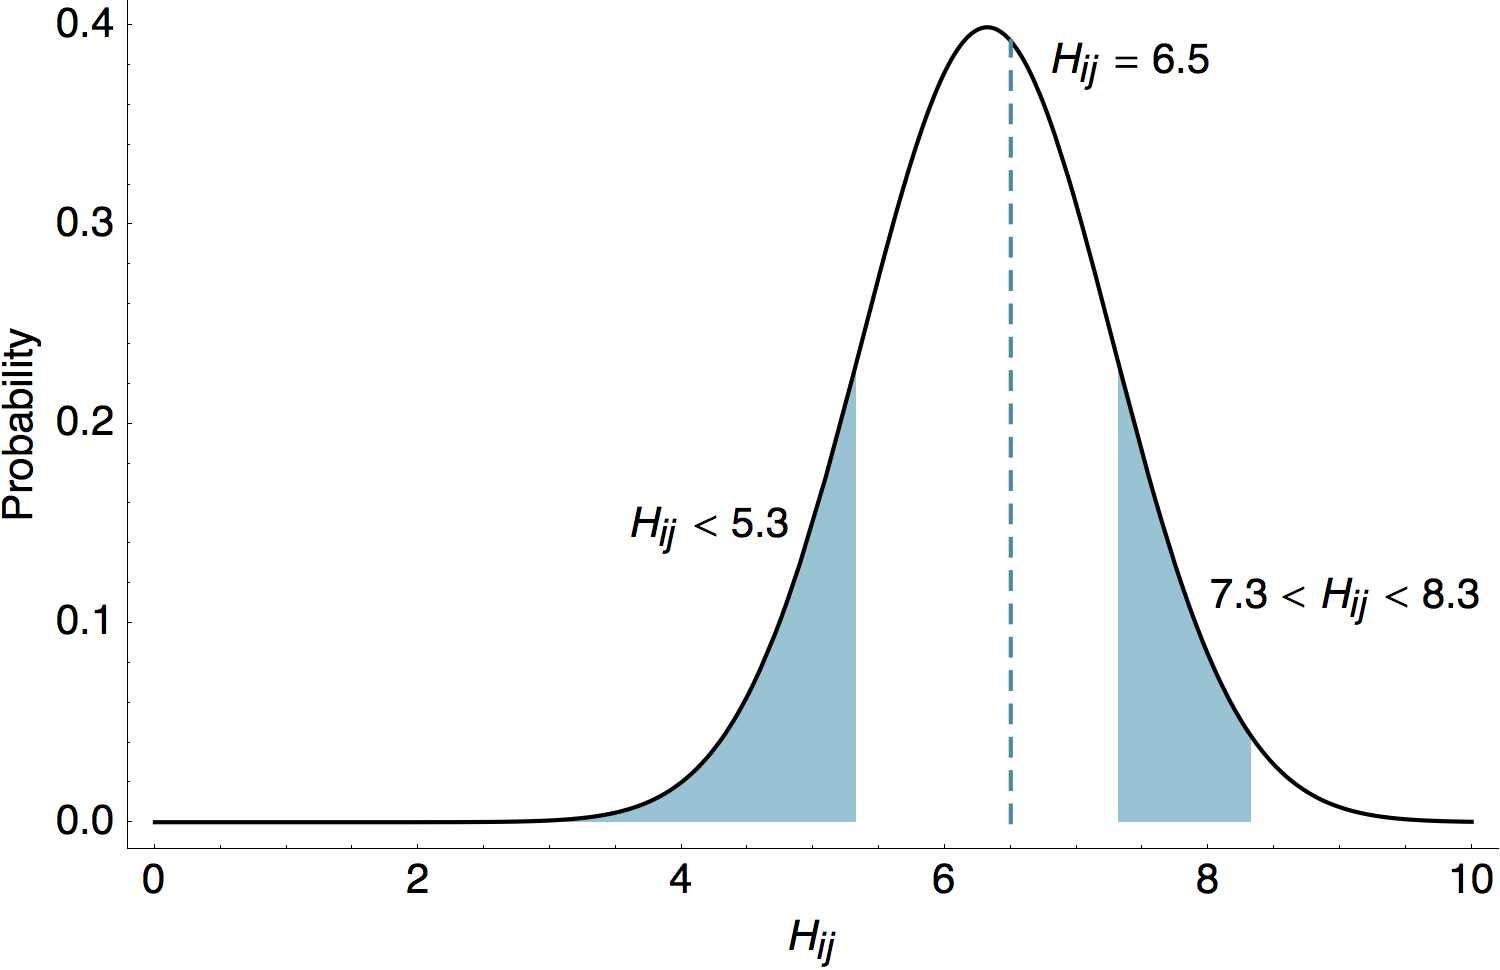
\includegraphics[width=0.6\textwidth]{figures/hij_likelihood}
	\caption{\textbf{Likelihood of HI titers in the BMDS model.} 
	Here we show the likelihoods of observing three different outcomes given $\delta_{ij} = 4$, $\mdssd = 0.95$ and $\se_j = \mathrm{log}_2 (1280) = 10.32$.  
	The likelihood of observing a threshold titer of `$<$40' is equal to the lower tail of the probability density function $\threshold(5.32) = 0.146$.
	The likelihood of observing a point measurement with an exact inhibiting titer of `90.5' is equal to the density function $\point(6.5) = 0.413$.
	The likelihood of observing an interval measurement with an inhibiting titer somewhere between `160' and `320' is equal to $\interval(7.32) = 0.129.$
	} 
	\label{hij_likelihood} 
\end{figure}

We calculate the overall likelihood by multiplying probabilities of individual measurements
\begin{equation} 
	L(\viruses,\sera) = \prod_{(i,j) \in \cal I} f(H_{ij}),
\end{equation}
using probability functions $\point$, $\threshold$ and $\interval$ as appropriate.
We begin by assuming independent, diffuse normal priors on virus and serum locations
\begin{eqnarray}
	\virus_i &\sim& \mathrm{Normal}(\boldsymbol{\mu},\boldsymbol{\Sigma}) \nonumber \\
	\serum_j &\sim& \mathrm{Normal}(\boldsymbol{\mu},\boldsymbol{\Sigma}),
\end{eqnarray}
where $\boldsymbol{\mu} = (0,\ldots,0)^{\prime}$ and $\boldsymbol{\Sigma}$ is a diagonal matrix with diagonal elements all equal to $10000$.

\subsection*{Virus and serum effects}

The preceding model represents immunological distance as a drop in titer against the most reactive comparison for a particular serum.
However, this model may be biased in some circumstances.
In one example, if a particular serum $j$ is only measured against distant viruses, its maximum titer will be artificially low and the likelihoods concerning this serum will appear poor. 
To address this issue, we relax the assumption of fixed $\se_j$ values and treat the expected log$_2$ titer when $\delta_{ij}=0$ as a random variable.
In this case, $H_{ij}$ still follows equation \ref{hij} with expectation $\se_j - \delta_{ij}$, but the vector of `serum effects' $\ses = (\se_1,\ldots,\se_{\sn})$ is random and estimated rather than fixed.
We assume that $\se_j$ values are hierarchically distributed according to a normal distribution.   
We take an Empirical Bayesian approach in specifying the mean and variance of this distribution, set to the empirical mean and empirical variance of the set of maximum titers across sera $\{ \max ( H_{1j},\ldots,H_{\vn j} ) : j = 1,\ldots,\sn \}$.
This formulation assumes that particular sera are more reactive in general than other sera.

Additionally, we follow the same logic and assume that some virus isolates are more reactive than other virus isolates and include a `virus effect' $\ve_i$ representing the general level of reactivity across HI assays. 
With virus reactivity included, observed titers follow
\begin{equation}
	H_{ij} \sim \normal \left( \frac{\ve_i+\se_j}{2} - \delta_{ij}, \, \mdssd^2 \right),
\end{equation}
and the vector of virus effects $\ve_i$ for $i = 1,\ldots, \vn$ is estimated in an analogous hierarchical fashion, with $\ves$ normally distributed with mean and variance equal to the empirical mean and variance of the set of maximum titers across viruses $\{ \max ( H_{i1},\ldots,H_{i \sn} ) : i = 1,\ldots,\vn \}$.

\subsection*{Drift model of antigenic evolution}

As presented, multiple configurations of virus and serum locations $\viruses$ and $\sera$ will give the same likelihood of an observed data matrix $\mathbf{H}$.
An example of this phenomenon is shown in Figure~\ref{schematic_map}.
In this case, it is impossible to determine from the HI data at hand whether the blue and yellow viruses are antigenically similar (Figure~\ref{schematic_map}A) or antigenically divergent (Figure~\ref{schematic_map}B). 
This presents an issue of model identifiability, where absolute, as opposed to relative, antigenic locations cannot be determined from the observing the serological data alone.
Thus, in order to achieve more a interpretable model we impose a weak prior on global locations.
In influenza, it's clear that antigenic distance between strains increases with time \cite{Smith04,Cai10}.
To capture this, we replace our previous diffuse prior with an informed prior in which the expected location of viruses and sera increases with date of sampling along dimension one, and each virus and serum location follows an independent normal distribution centered around this temporal expectation, so that
\begin{eqnarray}
	x_{i1} &\sim& \beta \, t_i + \normal(0, \virussd^2) \nonumber \\
	y_{j1} &\sim& \beta \, t_j + \normal(0, \serumsd^2),
\end{eqnarray}
where $t$ is the difference between the date of the indexed virus or serum and the date of the earliest sampled virus or serum, and other dimensions follow $x_{im} \sim \normal(0, \virussd^2)$ and $y_{jm} \sim \normal(0, \serumsd^2)$ for $m\ge2$.
Thus, this model assumes that virus and serum locations drift in a line across the antigenic map at rate $\beta$.
The parameter $\virussd$ determines the breadth of the cloud of virus locations at each point in time, while $\serumsd$ determines the breadth of the cloud of serum locations.

%%% schematic_map %%%
\begin{figure}[tb]
	\centering		
	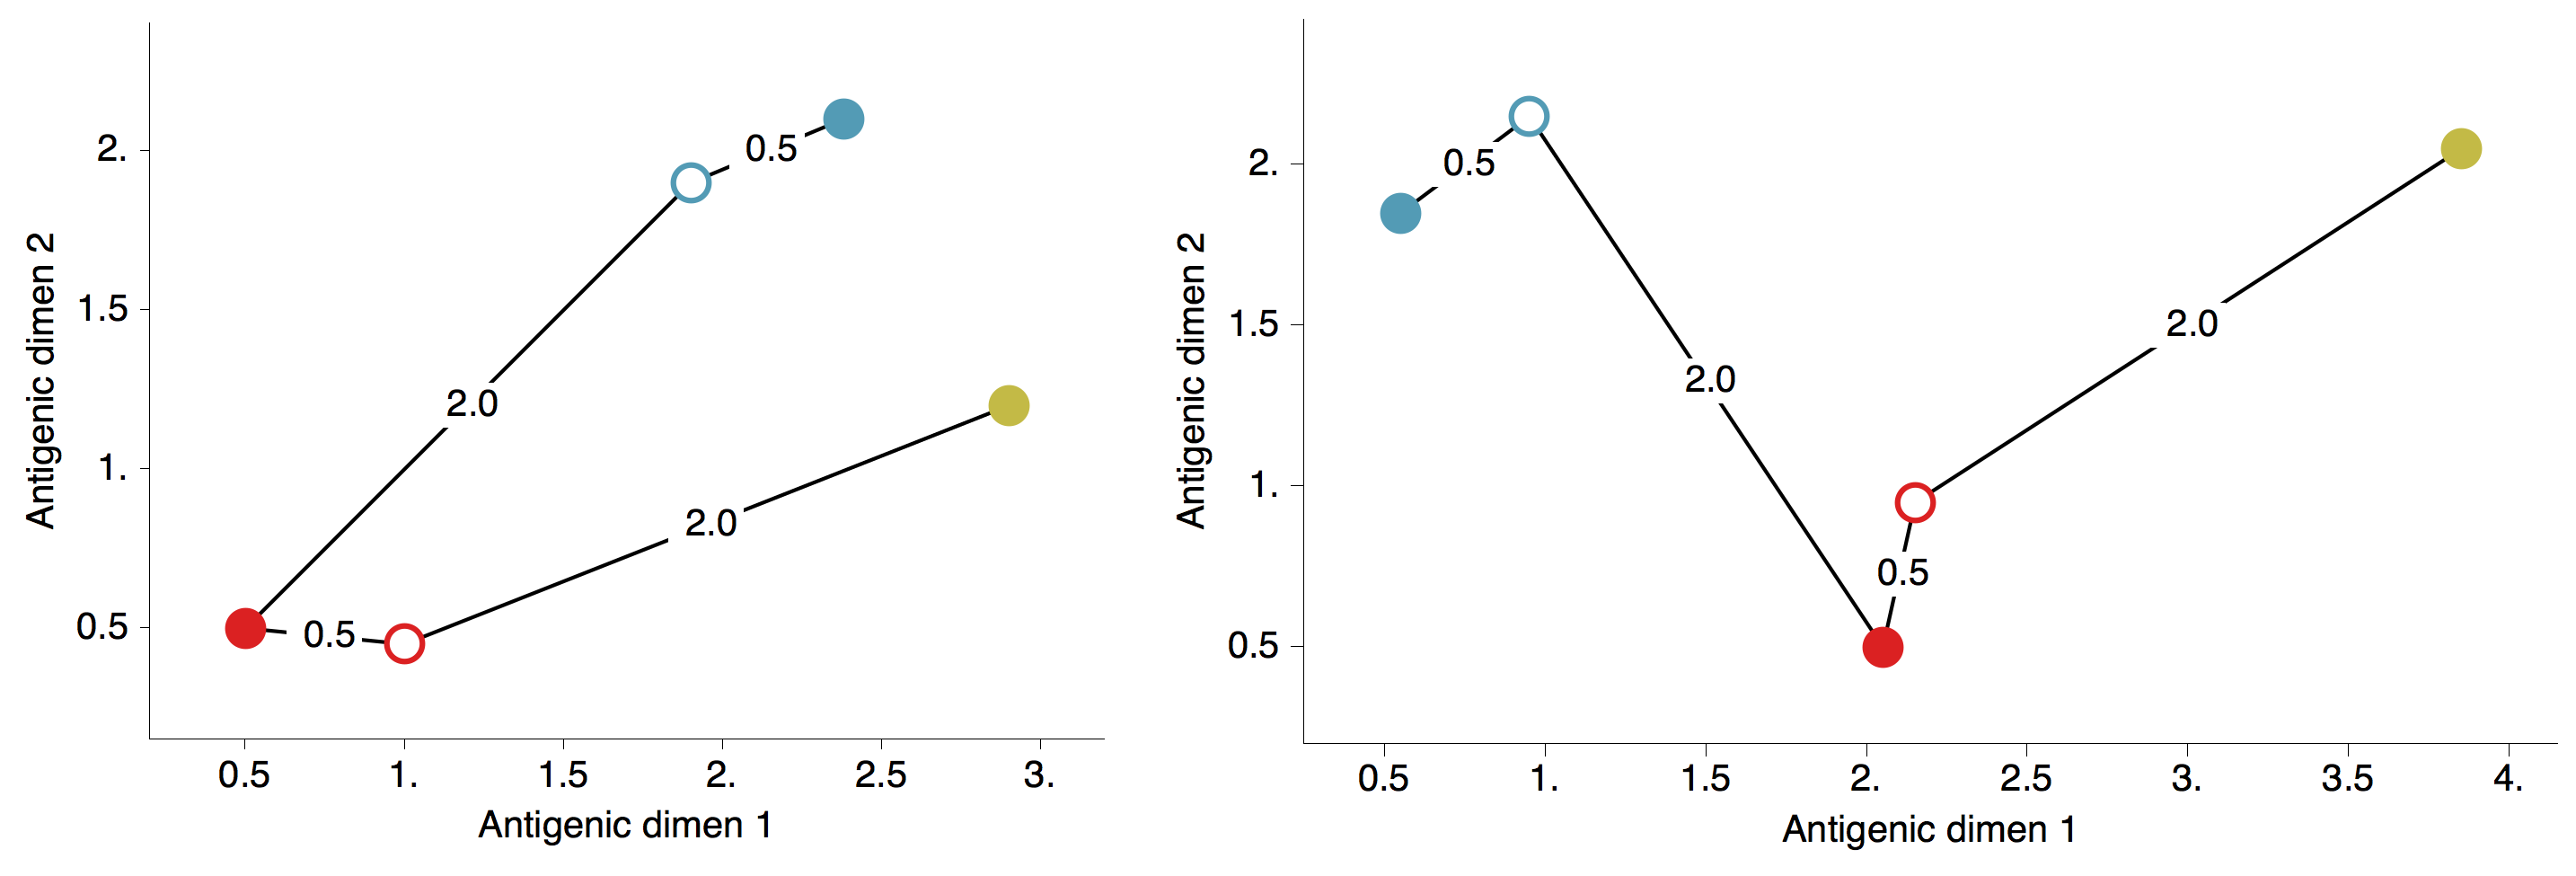
\includegraphics[width=0.95\textwidth]{figures/schematic_map}
	\caption{\textbf{Schematic antigenic map with three viruses and two sera.}
	(A) Map with virus 1 and virus 3 antigenically similar.
	(B) Map with virus 1 and virus 3 antigenically divergent.
	Virus 1 is shown in blue, virus 2 is shown in red and virus 3 is shown in yellow.
	Virus isolates are represented by filled circles, sera raised against viruses are shown as open circles and map distances $\delta_{ij}$ are shown as solid lines connecting viruses and sera.
	Sera from virus 1 is compared against viruses 1 and 2, while sera from virus 2 is compared against viruses 2 and 3.
	Configurations (A) and (B) represent cartographic models that would give equal likelihoods to a set of serological data $\{H_{11},H_{21},H_{22},H_{32}\}$.
	} 
	\label{schematic_map} 
\end{figure}

\subsection*{Phylogenetic diffusion model of antigenic evolution}

We simultaneously model antigenic locations and genetic relatedness by assuming that virus locations are influenced by evolution following a Brownian motion process \cite{Lemey10}.
To do this, we replace the previous prior specifying independent virus locations with a prior that incorporates covariance based on shared evolutionary history
\begin{equation} \label{ebpprior}
	\viruses \sim \left( \begin{matrix} \beta \, t_1 & 0 \\ \vdots & \vdots \\ \beta \, t_n & 0 \end{matrix} \right) + \, \mbox{Evolutionary Brownian Process}(\virussd, \tree)
\end{equation}
for $P=2$, where $\virussd$ is the volatility parameter of the Brownian motion and $\tree$ is a phylogeny specifying tree topology and branch lengths.
Thus, viruses which are genetically similar are induced to have prior locations close to one another on the antigenic map.
In the evolutionary Brownian process, the tips of the phylogeny $\tree$ correspond to the set of virus locations $(\virus_1, \ldots, \virus_\vn)$, and the probability of observing tip locations depends on the locations of internal nodes $(\virus_{n+1}, \ldots, \virus_{2\vn-2})$ and on the location of the root node $\virus_{2\vn-1}$.
This process assumes that a virus location $\virus_i$ follows from the location of its parent virus $\virus_{f(i)}$, and with the addition of drift along dimension 1, is distributed as
\begin{equation} 
	\virus_i \sim (\beta \, d_i, \, 0)^{\prime} + \normal(\virus_{f(i)}, d_i \, \boldsymbol{\Sigma})
\end{equation}
for $P=2$, where $f(i)$ is a function that maps nodes to parental nodes, $d_i$ is the length of the branch connecting virus $i$ to parent virus $f(i)$, and $\boldsymbol{\Sigma}$ is a diagonal matrix with diagonal elements all equal to $\virussd^2$.
The root virus location $\virus_{2\vn-1}$ is assumed to follow a normal distribution with expectation $(\beta \, t_{2\vn-1}, 0)^{\prime}$ for $P=2$ and variance determined by the diffusion volatility $\virussd$ \cite{Lemey10}.
The probability of virus locations $p(\viruses | \beta, \virussd, \tree)$ is determined through analytical integration across internal states following the methods introduced in \cite{Lemey10}.
This formulation corresponds to a Wiener process with drift, in which the drift term $\beta$ only influences the expected states of nodes along the phylogeny, but does not influence the covariance structure among these nodes, which remains the same as it does in a standard Wiener process \cite{BrownianMotionHandbook}.
This allows the separation in equation \ref{ebpprior} between drift terms affecting only expectations and the evolutionary Brownian process that includes covariance among virus locations $\virus_1,\ldots,\virus_n$.

Here, the phylogenetic tree $\tree$ is estimated using sequence data for viruses $1,\ldots,\vn$ according to well established methods implemented in the software package BEAST \cite{BEAST17}.

\subsection*{Posterior samples}

Top-level priors for $1/\mdssd^2$, $\beta$, $1/\virussd^2$, and $1/\serumsd^2$ are assumed to follow diffuse $\mbox{Gamma}(a, b)$ distributions  with $a=0.001$ and $b=0.001$.
Under the full model, the posterior probability of observing virus and serum locations given immunological data is factored
\begin{equation}
	p(\viruses,\sera | \mathbf{H}) \propto p(\mathbf{H} | \viruses, \sera, \ses, \ves, \mdssd) \; 
	p(\viruses | \beta, \virussd, \tree) \;
	p(\sera | \beta, \serumsd) \; 
	p(\ses, \ves, \mdssd, \beta, \virussd, \serumsd, \tree).
\end{equation}
We sample from this posterior distribution using the Markov chain Monte Carlo (MCMC) procedures implemented in the software package BEAST \cite{BEAST17}.
Metropolis-Hastings proposals include transition kernels that translate individual virus and serum locations $\virus_i$ and $\serum_j$ and individual virus effects $\ve_i$ and serum effects $\se_j$, and other transition kernels that scale the entire set of virus and serum locations $\viruses$ and $\sera$ and that scale parameters $\mdssd$, $\beta$, $\virussd$ and $\serumsd$.
For the present analysis, a two-step approach was taken to sample phylogenies, where a posterior sample of phylogenies was gathered using sequence data and then, in the cartographic analysis, trees from this set were randomly proposed and accepted following the Metropolis-Hastings algorithm \cite{Pagel04}.

\subsection*{Genetic, antigenic and surveillance data}

We compiled an antigenic dataset of hemagglutination inhibition (HI) measurements of virus isolates against post-infection ferret sera for influenza A/H3N2 by collecting data from previous publications \cite{Hay01,Smith04,Russell08,Barr10}, NIMR vaccine strain selection reports for 2002 and 2008--2012 \cite{NIMR02,NIMRMarch08,NIMRFeb09,NIMRFeb10,NIMRSep10,NIMRSep11,NIMRFeb12} and the Feb 2011 VRBPAC report \cite{Cox11FDA}.
We queried the Influenza Research Database \cite{IRD} and the EpiFlu Database \cite{GISAID} for HA nucleotide sequences by matching strain names, e.g.\ A/HongKong/1/1968, and only strains for which sequence was present was retained.
If a strain had multiple sequences in the databases we preferentially kept the IRD sequence and preferentially kept the longest sequence in IRD. 
Sequences were aligned using MUSCLE v3.7 under default parameters \cite{MUSCLE}.
This dataset had 2051 influenza isolates (present as either virus or serum in HI comparisons) dating from 1968 to 2011. 
However, the majority of isolates were present from 2002 to 2007. 
Because we are interested in longer-term antigenic evolution, we subsampled the data to have at most 20 virus isolates per year, preferentially keeping those isolates with more antigenic comparisons. 
We then kept only those serum isolates that are relatively informative to the antigenic placement of viruses, dropping serum isolates that are compared to 4 or fewer different virus isolates.
This censoring left 402 virus isolates, 519 serum isolates and 10,059 HI measurements. 

Antigenic data for influenza A/H1N1 was collected from previous publications \cite{Kendal78,Webster79,Nakajima79,Nakajima81,Chakraverty82,Pereira82,Chakraverty86,Cox83,Daniels85,Raymond86,Stevens87,Donatelli93,Hay01,Daum02,McDonald07,Barr10} and NIMR vaccine strain selection reports for 2002--2010 \cite{NIMR02,NIMR03,NIMR04,NIMRFeb05,NIMRSep05,NIMRMarch06,NIMRSep06,NIMRMarch07,NIMRSep07,NIMRMarch08,NIMRSep08,NIMRFeb09,NIMRFeb10}.
The same procedure was followed as was followed for H3N2 to match sequence data and to subsample antigenic comparisons.
This procedure yielded 115 virus isolates, 77 serum isolates and 1882 HI measurements over the course of 1977 to 2009.

Antigenic comparisons for influenza B/Victoria were collated from previous publications \cite{Rota90, Hay01, Muyanga01, Shaw02, Ansaldi04, Puzelli04, Xu04, Barr06, Daum06, Lin07} and vaccine strain selection reports for 2002--2012 \cite{AusWHO06, NIMR02, NIMR03, NIMR04, NIMRFeb05, NIMRSep05, NIMRMarch06, NIMRSep06, NIMRMarch07, NIMRSep07, NIMRMarch08, NIMRFeb09, NIMRSep09, NIMRFeb10, NIMRSep10, NIMRFeb11, NIMRSep11, NIMRFeb12}.
Here, the sequence matching and subsampling procedure yielded 179 virus isolates, 70 serum isolates and 2003 HI measurements over the course of 1986 to 2011.

Antigenic comparisons for influenza B/Yamagata were collected from previous publications \cite{Rota90, Kanegae90, Nakajima92, Nerome98, Hay01, Muyanga01, Nakagawa02, Abed03, Ansaldi03, Ansaldi04, Matsuzaki04, Puzelli04, Shaw02, Xu04, Barr06, Daum06, Lin07} and vaccine strain selection reports for 2002--2012 \cite{AusWHO06, NIMR02, NIMR03, NIMR04, NIMRFeb05, NIMRSep05, NIMRMarch06, NIMRSep06, NIMRMarch07, NIMRSep07, NIMRMarch08, NIMRFeb09, NIMRSep09, NIMRFeb10, NIMRSep10, NIMRFeb11, NIMRSep11, NIMRFeb12}.
For B/Yamagata, the matching and subsampling procedure resulted in 174 virus isolates, 69 serum isolates and 1962 HI measurements over the course of 1987 to 2011.

Surveillance data was obtained from the Centers of Disease Control and Prevention FluView Influenza Reports from the yearly summaries of influenza seasons 1997--1998 to 2010--2011 \cite{CDCReports}.
As an example, one report states ``collaborating laboratories in the United States tested 195,744 respiratory specimens for influenza viruses, 27,682 (14\%) of which were positive. Of these, 18,175 (66\%) were positive for influenza A viruses, and 9,507 (34\%) were positive for influenza B viruses. Of the 18,175 specimens positive for influenza A viruses, 7,631 (42\%) were subtyped; 6,762 (87\%) of these were seasonal influenza A (H1N1) viruses, and 869 (13\%) were influenza A (H3N2) viruses.''
In this case, we estimate the relative proportion of A/H3N2 of the four clades as $0.66 \times 0.13 = 0.09$.
Similar calculations were performed for A/H1N1, B/Vic and B/Yam.

\subsection*{Implementation}

Phylogenetic trees were estimated for A/H3N2, A/H1N1, B/Vic and B/Yam using BEAST \cite{BEAST17} and incorporated the SRD06 nucleotide substitution model \cite{Shapiro06}, a coalescent demographic model with constant effective population size and a strict molecular clock across branches.
MCMC was run for 60 million steps and trees were sampled every 50,000 steps after allowing a burn-in of 10 million steps, yielding a total sample of 2000 trees.
These trees were treated as a discrete set of possibilities when subsequently sampled in the BMDS analysis \cite{Pagel04}.
However, it would be possible to jointly sample from sequence data and serological data using these methods.

MCMC was used to sample virus locations $\viruses$, serum locations $\sera$, virus effects $\ves$, serum effects $\ses$, MDS precision $1/\mdssd^2$, antigenic drift rate $\beta$, virus location precision $1/\virussd^2$, serum location precision $1/\serumsd^2$ and phylogenetic tree $\tree$.
MCMC chains were run for 500 million steps and parameter values sampled every 200,000 steps after a burn-in of 100 million steps, yielding a total of 2000 MCMC samples.

There is some difficulty summarizing posterior cartographic samples, as sampled virus and serum locations represent only relative quantities, and because of this, over the course of the MCMC, virus locations may shift.
Our prior on virus and serum locations removes much of this issue, orienting the antigenic map along dimension 1 and fixing it to begin at the origin.
However, local isometries are often still a problem.
For example, in A/H3N2 the Beijing/89 cluster may shift back and forth from being above other viruses on dimension 2 to being below other viruses on dimension 2.
These isometries may be local, i.e.\ Beijing/89 and Beijing/92 may flip while leaving Victoria/75 in place.
Consequently, it is difficult to fully align MCMC samples using Procrustes analysis.
For the present study, we take a simple approach and sample a single MCMC step and visualize the antigenic locations at this state (Figures~1, Figure~2).
Then, for specific quantities of interest, like rate of antigenic drift and rate of diffusion at different points along the phylogeny, we calculate this quantity across MCMC samples to yield an expectation and a credible interval.
This approach accurately characterizes uncertainty that may be hidden in an analysis of a single antigenic map.

\subsection*{Estimation of diffusion coefficient}

The distance $d$ traveled by a diffusion is not a linear function of time interval $t$, and thus the `rate' of diffusion cannot be calculated following $r=d/t$.
Assume we have a one-dimensional diffusion starting from $x_0 = 0$, so that
\begin{equation}
	X_t \sim \normal(0, \sigma^2 t),
\end{equation}
where $\sigma$ represents the diffusion volatility, and in this case, the expected squared displacement follows
\begin{equation}
	\mathrm{E}[X_t^2] = \sigma^2 t.
\end{equation}
In moving to a two-dimensional diffusion
\begin{equation}
	(X_t, Y_t) \sim \normal \left( \twomatrix{0}{0}, \fourmatrix{\sigma_x^2 t}{\rho \sigma_x \sigma_y t}{\rho \sigma_x \sigma_y t}{\sigma_y^2 t} \right),
\end{equation}
where $\sigma_x$ represents volatility in dimension 1, $\sigma_y$ represents volatility in dimension 2 and $\rho$ represents correlation,   expected squared displacement is equal to the sum of squared displacements in each dimension
\begin{equation}
	\mathrm{E}[X_t^2 + Y_t^2] = \sigma_x^2 t + \sigma_y^2 t.
\end{equation}
Such diffusions are often characterized with diffusion coefficient $D$.
In this case
\begin{equation}
	D = \frac{\sigma_x^2 + \sigma_y^2}{4},
\end{equation}
so that expected squared displacement follows from $D$ alone
\begin{equation}
	\mathrm{E}[X_t^2 + Y_t^2] = 4 D t.
\end{equation}

Owing to this relationship, Pybus et al.\ \cite{Pybus12} estimate $D$ from phylogenies in which internal nodes have inferred 2D locations via the formula
\begin{equation} \label{pybusest}
	\hat{D} = \frac{1}{n} \sum^n_{i=1} \frac{d_i^2}{4t_i},
\end{equation}
in which $d_i$ represents the displacement of a branch and $t_i$ represents the length of a branch.
However, uncertainty in $d_i$ or $t_i$, especially along short branches of the phylogeny, may cause $d_i^2/4t_i$ to have high variance and increase uncertainty in the resulting estimates of $D$.
Consequently, we estimate $D$ by looking at the relationship between total squared displacement and total time along branches of a phylogeny
\begin{eqnarray} \label{ourest}
	d^2_\Sigma &=& \sum^n_{i=1} d^2_i \nonumber \\
	t_\Sigma &=& \sum^n_{i=1} t_i \nonumber \\
	\hat{D} &=& \frac{ d^2_\Sigma }{ 4 t_\Sigma }.
\end{eqnarray}
This estimator showed less variance than equation \ref{pybusest} when analyzing tree output from the BMDS model and was thus preferred.
Additionally, we confirmed through simple simulation that estimator \ref{ourest} shows lower mean squared error than estimator \ref{pybusest} in the presence of modest levels of noise on estimates of $d_i$ and $t_i$.
When estimating $D$ specific to trunk branches or specific to side branches, we calculate $d^2_\Sigma$ and $t_\Sigma$ only from a subset of phylogeny branches as appropriate.

%%% REFERENCES %%%
\bibliographystyle{plos}
\bibliography{flux}

\end{document}